 \documentclass[11pt]{article}
\usepackage{geometry, titlesec}
\usepackage[parfill]{parskip}
\usepackage[italicdiff]{physics}
\usepackage{amsfonts, amsthm}
\usepackage[cm]{fullpage}
\usepackage{fancyhdr}
\usepackage{enumitem}
\usepackage{xcolor, soul}
\usepackage{kbordermatrix}
%\allowdisplaybreaks

\makeatletter
\renewcommand*\env@cases[1][1.2]{%
  \let\@ifnextchar\new@ifnextchar
  \left\lbrace
  \def\arraystretch{#1}%
  \array{@{}l@{\quad}l@{}}%
}
\makeatother

 
\renewcommand{\footrulewidth}{.2pt}
%\setlist[enumerate]{leftmargin=*}
\pagestyle{fancy}
\fancyhf{}
\lhead{\textbf{Physics 342 Homework 1}}
\rhead{Lacey Rainbolt}
\setlength{\headheight}{11pt}
\setlength{\headsep}{11pt}
\setlength{\footskip}{24pt}
\lfoot{\today}
\rfoot{\thepage}

\titleformat{\section}[runin]{\normalfont\large\bfseries}{Problem \thesection.}{1em}{}
\titleformat{\subsection}[runin]{\normalfont\large\bfseries}{\thesubsection}{1em}{}
\titleformat{\subparagraph}[leftmargin]{\normalfont\normalsize\bfseries}{}{0pt}{}

\newcommand{\refeq}[1]{(\ref{#1})}

\newcommand{\beq}{\begin{equation*}}
\newcommand{\eeq}{\end{equation*}}

\newcommand{\beqn}{\begin{equation}}
\newcommand{\eeqn}{\end{equation}}


\renewcommand{\vec}[1]{\mathbf{#1}}
\newcommand{\vfix}{\vspace{-\baselineskip}}


\newenvironment{statement}[1]
{
	\section{#1}
	\color{darkgray}
	\ignorespaces
}
{
%    \smallskip
}

\newenvironment{problem}
{
    \color{darkgray}
    \subsection{}
    \ignorespaces
}


\newenvironment{solution}
{
    \paragraph{Solution.}
    \ignorespaces
}
{
%    \smallskip
}

\newcommand{\Schrodinger}{Schr\"{o}dinger}


\begin{document}

\state{Spin-wave theory~(P\&S 11.1)}{\hfix}

\prob{ \label{1a}
	Prove the following wonderful formula: Let $\phix$ be a free scalar field with propagator $\ev{T \phix \phio} = \Dx$.  Then
	\eqn{show1}{
		\ev{ T e^{i \phix} e^{-i \phio} } = e^{[ \Dx - \Do ]}.
	}
	(The  factor $\Do$ gives a formally divergent adjustment of the overall normalization.)
}

\sol{
	According to P\&S~(9.18),
	\eq{
		\ev*{T \phi(\xq) \phi(\xw)}{\Omg} = \frac{\int \DDphi \phi(\xq) \phi(\xw) \exp[ i \int \ddqx \cL ]}{\int \DDphi \exp[ i \int \ddqx \cL ]}.
	}
	We use this expression to write the left-hand side of Eq.~\refeq{show1}:
	\eqn{thing1}{
		\ev{ T e^{i \phix} e^{-i \phio} } = \frac{\int \DDphi e^{i \phix} e^{-i \phio} \exp[ i \int \ddqy \cL ]}{\int \DDphi \exp[ i \int \ddqy \cL ]}
		= \frac{\int \DDphi \exp[i \phix - i \phio + i \int \ddqy \cL ]}{\int \DDphi \exp[ i \int \ddqy \cL ]}.
	}
	For a free Klein-Gordon~(i.e., scalar) field, Eq.~(9.39) tells us that the generating functional $\ZJ$ is given by
	\eq{
		\ZJ = \Zo \exp[ -\frac{1}{2} \int \ddqx \ddqy \Jx \DF(x - y) \Jy ],
	}
	where $\Zo = Z[0]$.  Thus, we want to find some $\Jy$ such that
	\eqn{thing1b}{
		\ev{ T e^{i \phix} e^{-i \phio} } = \frac{\ZJ}{\Zo}
	}
	where in general
	\eq{
		\ZJ = \int \DDphi \exp[ i \int \ddqx [ \cL + \Jx \phi(x) ] ]
	}
	by (9.34).  Inspecting Eq.~\refeq{thing1}, we recognize the denominator as $\Zo$ and see that if
	\eq{
		\Jy = \delq(y - x) - \delq(y)
	}
	we have an expression like Eq.~\refeq{thing1b}.  Collecting these findings, we have
	\al{
		\ans{ \ev{ T e^{i \phix} e^{-i \phio} } }&= \frac{\ZJ}{\Zo} \\
		&= \exp[ -\frac{1}{2} \int \ddqy \ddqz \Jy \DF(y - z) \Jz ] \\
		&= \exp[ -\frac{1}{2} \int \ddqy \ddqz \Jy \DF(y - z) [ \delq(z - x) - \delq(z) ] ] \\
		&= \exp[ -\frac{1}{2} \int \ddqy [ \delq(y - x) - \delq(y) ] [ \DF(y - x) - \DF(y) ] ] \\
		&= \exp[ -\frac{1}{2} [ \DF(0) - \DF(x) - \DF(-x) + \DF(0) ] ] \\
		&= \exp[ \DF(x) - \DF(0) ] \\
		&\ans{\; = e^{[ \Dx - \Do ]}, }
	}
	as we wanted to show. \qed
}



\prob{ \label{1b}
	We can use this formula in Euclidean field theory to discuss correlation functions in a theory with spontaneously broken symmetry for $T < \TC$.  Let us consider only the simplest case of a broken $O(2)$ or $U(1)$ symmetry.  We can write the local spin density as a complex variable
	\eq{
		\sx = \sqx + i \swx.
	}
	The global symmetry is the transformation
	\eq{
		\sx \to e^{-i \alp} \sx.
	}
	If we assume that the physics freezes the modulus of $\sx$, we can parameterize
	\eqn{sx}{
		\sx = A e^{i \phix}
	}
	and write an effective Lagrangian for the field $\phix$.  The symmetry of the theory becomes the translation symmetry
	\eqn{symmetry}{
		\phix \to \phix - \alp.
	}
	Show that (for $d > 0$) the most general renormalizable Lagrangian consistent with this symmetry is the free field theory
	\eqn{show1b}{
		\cL = \frac{1}{2} \rho(\vgrad \phi)^2.
	}
	In statistical mechanics, the constant $\rho$ is called the \emph{spin wave modulus}.  A reasonable hypothesis for $\rho$ is that it is finite for $T < \TC$ and tends to 0 as $T \to \TC$ from below.
}

\sol{
	In accordance with the Klein-Gordon Lagrangian in P\&S~(2.6),
	\eqn{KGL}{
		\cL_\text{K-G} = \frac{1}{2} (\pt \phi)^2 - \frac{1}{2} m^2 \phi^2,
	}
	we interpret $(\vgrad \phi)^2$ as $(\pt \phi)^2$.
	
	The Lagrangian cannot have terms of $\order{\phi^n}$ for any $n \neq 0$ since $\phi(x)$ is not invariant under Eq.~\refeq{symmetry}.  Any combination of derivatives of $\phi$ is invariant, however, since $\alp$ is a constant and does not contribute to any derivative.  Thus, only terms like $\pt^n \phi^m$ (where $n$ denotes a power of $\pt$) for $n, m > 0$ and $n \geq m$ are consistent with the symmetry of Eq.~\refeq{symmetry} for $d$ an integer.
	
	Now we must determine which of these terms are renormalizable.  We know that the Lagrangian must have dimension $d$, and that $\phi$ has dimension $(d - 2) / 2$.  Taking a derivative adds a mass dimension.  The theory is renormalizable if the coupling constant $\rho$ has dimension greater than or equal to 0~\cite[p.~322]{Peskin}.  Let $p$ be the dimension of $\rho$.  The dimension of our allowed term is then
	\eq{
		[ \rho \pt^n \phi^m ] = p + n + m \frac{d - 2}{2},
	}
	which we require to be equal to $d$.  Thus we seek solutions to the system of equations
	\al{
		d &= p + n + m \frac{d - 2}{2}, &
		n &\geq m, &
		p &\geq 0.
	}
	Solving with Mathematica, we find that this system has two solutions: $n = m = 2$ and $p = 0$; and $n = m = 1$ and $p = d / 2$.  However, the term $\pt \phi$ for $n = m = 1$ does not contribute to the action because it is a total derivative and does not contribute when the integral over $\cL$ is evaluated:
	\eq{
		\int \dd[d]{x} \pt\phi = \phi \bigg|_{-\infty}^\infty
		= 0.
	}
	Thus the only possibility is $n = m = 2$.  Note that
	\eq{
		\pt^2 \phi^2 = \pt(\pt \phi^2)
		= 2 \pt( \phi \pt \phi)
		= \pt \phi \pt \phi + \phi \pt^2 \phi
		= (\pt \phi)^2,
	}
	since $\phi \pt^2 \phi$ is not invariant under Eq.~\refeq{sx}.  This means that $\rho$ must be dimensionless and that the only allowed terms in the Lagrangian are proportional to $(\pt \phi)^2$, which is consistent with Eq.~\refeq{show1b}. \qed
}



\prob{
	Compute the correlation function $\ev{ \sx \sao }$.  Adjust $A$ to give a physically sensible normalization (assuming that the system has a physical cutoff at the scale of one atomic spacing) and display the dependence of this correlation function on $x$ for $d = 1, 2, 3, 4$.  Explain the significance of your results.
}

\sol{
	Applying Eq.~\refeq{sx},
	\eq{
		\ev{ \sx \sao } = \ev*{ A e^{i \phix} \As e^{-i \phio} }
		= \ev*{ \abs{A}^2 } \ev*{ e^{i \phix} e^{-i \phio} }.
	}
	Now we can apply Eq.~\refeq{show1} to find
	\eqn{thing1c}{
		\ans{ \ev{ \sx \sao } = \abs{A}^2 \exp[ D(x) - D(0) ], }
	}
	where $D(x - y)$ is a Green's function.  Since our Lagrangian is similar to the Klein-Gordon Lagrangian Eq.~\refeq{2.6}, our Green's function is similar to that of the Klein-Gordon operator, which is given by P\&S~(2.56):
	\eq{
		(\pt^2 + m^2) D(x - y) = -i \delq(x - y).
	}
	The Feynman prescription for this Green's function is given by (2.59),
	\eqn{DF}{
		\DF(x - y) = \int \ddqpf \frac{i}{p^2 - m^2 + i \eps} e^{-i p \cdot (x - y)}.
	}
	For the Lagrangian in Eq.~\refeq{show1b}, we set $m = 0$ and insert a factor of $\rho$:
	\eq{
		\rho \pt^2 D(x - y) = -i \deld(x - y),
	}
	so adapting Eq.~\refeq{DF} for this situation yields
	\eqn{DF}{
		\DF(x - y) = \frac{1}{\rho} \int \dddpf \frac{i}{p^2 + i \eps} e^{-i p \cdot (x - y)}.
	}
	We see that $\DF(0)$ diverges, so we absorb it into the constant to make the normalization physically sensible.  We can do this because, as we showed in \ref{1b}, the theory is renormalizable.  Define $A'$ such that
	\eq{
		{A'}^2 = \abs{A}^2 e^{-D(0)}.
	}
	Then Eq.~\refeq{thing1c} can be written
	\eq{
		\ans{ \ev{ \sx \sao } =  {A'}^2 e^{D(x)}. }
	}
	
	To evaluate the divergent integral $D(x)$, we look to the Feynman parameter method we have been using to solve divergent integrals.  Apparently, the Schwinger parametrization is useful in deriving the Feynman parametrization, and it is given by~\cite{Feynman}
	\eq{
		\frac{1}{A} = \intoi \dds e^{-s A}.
	}
	Using this equation, we can write Eq.~\refeq{DF} as
	\eq{
		\DF(x) = \frac{1}{\rho} \int \dddpf \frac{i}{p^2} e^{-i p \cdot x}
		= \frac{i}{\rho} \int \dddpf \intoi \dds e^{-s p^2} e^{-i p \cdot x}.
	}
	Now we can complete the square in the exponential to get a Gaussian integral:
	\al{
		\DF(x) &= \frac{i}{\rho} \int \dddpf \intoi \dds \exp[ -s p^2 - i p \cdot x + \frac{x^2}{4 s} - \frac{x^2}{4 s} ] \\
		&= \frac{i}{\rho} \int \dddpf \intoi \dds \exp[ -s \paren{ p + \frac{i x}{2 s} }^2 - \frac{x^2}{4 s} ] \\
		&= \frac{i}{\rho (2 \pi)^d} \intoi \dds e^{-x^2 / 4 s} \int \dd[d]{u} e^{-s u^2} \\
		&= \frac{i}{\rho (2 \pi)^{d}} \intoi \dds e^{-x^2 / 4 s} \sqrt{ \frac{(2\pi)^d}{(2s)^d} } \\
		&= \frac{i}{\rho (4 \pi)^{d / 2}} \intoi \dds \frac{e^{-x^2 / 4 s}}{s^{d / 2}}
	}
	where we have used~\cite{QFT}
	\eq{
		\int \exp( -\frac{1}{2} x \cdot A \cdot x ) \dd[n]{x} = \sqrt{\frac{(2\pi)^n}{\det A}},
	}
	with $A$ a $d \times d$ diagonal matrix $2s$.  Using Mathematica to integrate with respect to $s$, we find
	\eq{
		\DF(x) = \frac{i}{\rho (4 \pi)^{d / 2}} \frac{2^{d - 2}}{x^{d - 2}} \Gam(d / 2 - 1)
		= \frac{i}{4 \pi^d \rho} \Gam(d / 2 - 1) x^{2 - d}.
	}
	The gamma function diverges as $d \to 2$, so as we have done in previous problems, we expand about $\eps = 2 - d$.  Evaluating the series expansion using Mathematica, we obtain
	\eq{
		\DF(x) = \frac{i}{4 \pi^{1 - \eps} \rho} \Gam(\eps / 2) x^\eps
		\approx \frac{i}{4 \pi \rho} \paren{ \frac{2}{\eps} - \gam + 2 \ln(\pi x) }
		\sim \frac{i}{2 \pi \rho} \ln(x)
		= i \ln(\frac{1}{x^{2 \pi \rho}}).
	}
	We Wick rotate $x \to i x$.  Then the dependence of the correlation function on $x$ for $d = 1, 2, 3, 4$ is
	\ans{\al{
		(d = 1) &\qquad \ev{ \sx \sao } \sim e^{-x / 2 \sqrt{\pi} \rho}, &
		(d = 2) &\qquad \ev{ \sx \sao } \sim x^{2 \pi \rho}, \\
		(d = 3) &\qquad \ev{ \sx \sao } \sim \frac{1}{x}, &
		(d = 4) &\qquad \ev{ \sx \sao } \sim \frac{1}{x^2}.
	}}%
	In $d > 2$ dimensions, the expectation value of the correlation function tends to 0 at large distances $x$.  For $d > 2$, it drops off more quickly as $d$ increases.  The $d \leq 2$ cases depend on $\rho$, which we assume is positive.  The $d = 1$ case drops off with increasing distance, and more quickly with smaller $\rho$.  For $d = 2$, the expectation value of the correlation function increases with increasing distance, and it blows up more quickly with larger $\rho$.
	
	These results are consistent with the Mermin--Wagner theorem, which states that a continuous symmetry cannot be broken in $d \leq 2$ dimensions~\cite{CMW}.  That is, in $d \leq 2$ dimensions, a symmetry-breaking field cannot have a nonzero vacuum expectation value~\cite[p.~460]{Peskin}.  A physical explanation is that each spin has more nearest neighbors in higher dimensions.  Since the spins are inclined to align with their neighbors, there is a higher degree of correlation in higher dimensions at the same distance.  In two dimensions, the correlations are weak enough that they are overpowered by the field fluctuations.
}

\newcommand{\Fab}{F^{\alp \bet}}
\newcommand{\Ua}{U^\alp}
\newcommand{\Usa}{U_\alp}
\newcommand{\Ub}{U^\bet}
\newcommand{\Xa}{X^\alp}
\newcommand{\Xsa}{X_\alp}
\newcommand{\Xb}{X^\bet}
\newcommand{\xap}{x^\alp_p}
\newcommand{\xaq}{x^\alp_q}

\begin{statement}{(Jackson 11.17)}
	The electric and magnetic fields \refeq{fields} of a charge in uniform motion can be obtained from Coulomb's law in the charge's rest frame and the fact that the field strength $\Fab$ is an antisymmetric tensor of rank 2 without considering \emph{explicitly} the Lorentz transformation.  The idea is the following.  For a charge in uniform motion the only relevant variables are the charge's 4-velocity $\Ua$ and the relative coordinate $\Xa = \xap - \xaq$, where $\xap$ and $\xaq$ are the 4-vector coordinates of the observation point and the charge, respectively.  The only antisymmetric tensor that can be formed is $(\Xa \Ub - \Xb \Ua)$.  Thus the electromagnetic field $\Fab$ must be this tensor multiplied by some scalar function of the possible scalar products, $\Xsa \Xa$, $\Xsa \Ua$, $\Usa \Ua$.
\end{statement}

\newcommand{\vbb}{\vb{b}}
\newcommand{\vv}{\vb{v}}
\newcommand{\Eq}{E_1}
\newcommand{\Ew}{E_2}
\newcommand{\Ee}{E_3}
\newcommand{\Bq}{B_1}
\newcommand{\Bw}{B_2}
\newcommand{\Be}{B_3}

\newcommand{\xsq}{x^1}


\begin{figure} \centering
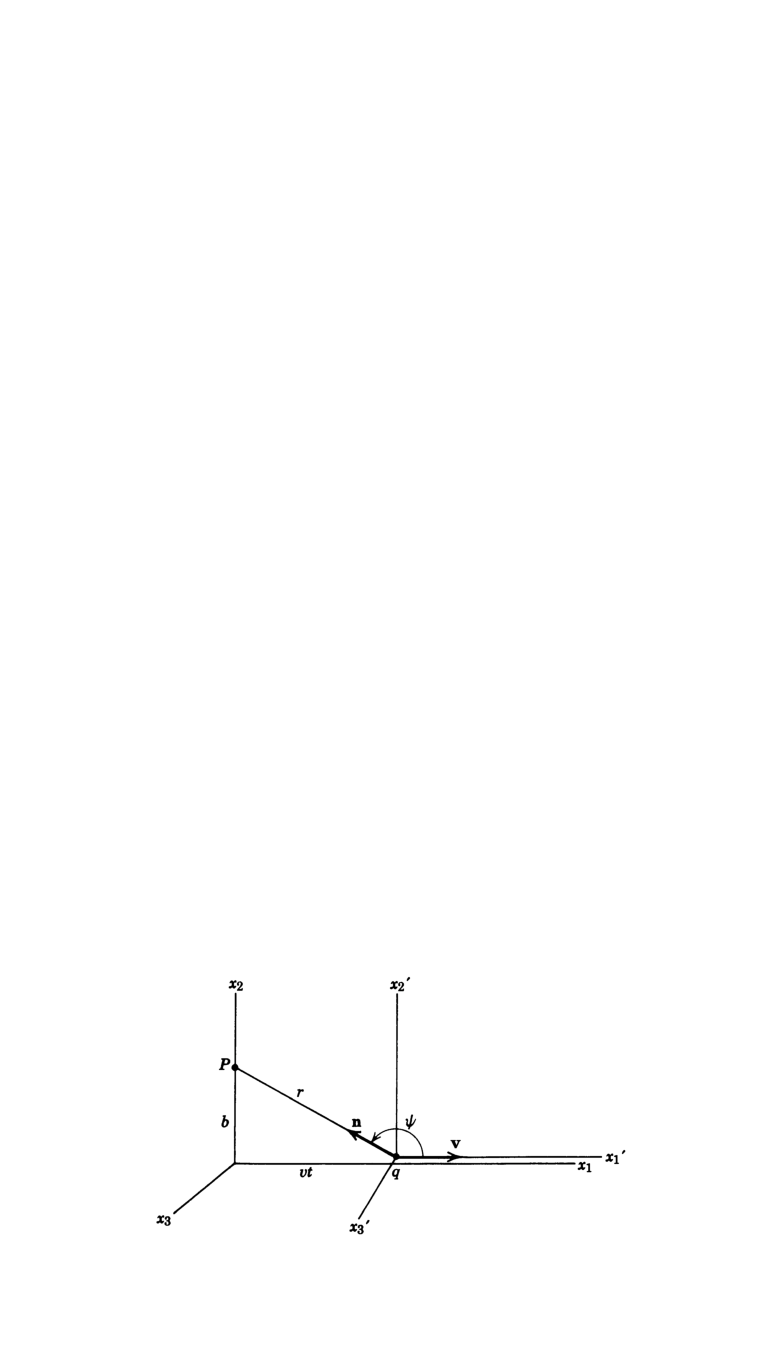
\includegraphics{11-8}
\caption{(Jackson Fig.~11.8) Particle of charge $q$ moving at constant velocity $\vv$ passes an observation point $P$ at impact parameter $b$.}
\label{11.8}
\end{figure}

\begin{problem} \label{2.a}
	For the geometry of Fig.~\ref{11.8} the coordinates of $P$ and $q$ at a common time in $K$ can be written $\xap = (ct, \vbb)$, $\xaq = (ct, \vv t)$, with $\vbb \vdot \vv = 0$.  By considering the general form of $\Fab$ in the rest frame of the charge, show that
	\beqn \label{show2.a}
		\Fab = \frac{q}{c} \frac{\Xa \Ub - \Xb \Ua}{[(\Usa \Xa / c)^2 - \Xsa \Xa]^{3/2}}.
	\eeqn
	Verify that this yields the expressions
	\begin{align} \label{fields}
		\Eq &= \Eq' = -\frac{q \gam v t}{(b^2 + \gam^2 v^2 t^2)^{3/2}}, &
		\Ew &= \gam \Ew' = \frac{\gam q b}{(b^2 + \gam^2 v^2 t^2)^{3/2}}, &
		\Be &= \gam \bet \Ew' = \bet \Ew,
	\end{align}
	with all other components vanishing, in the inertial frame $K$.
\end{problem}


\newcommand{\Fmat}{\mqty[	0 & -\Eq & -\Ew & -\Ee \\
						\Eq & 0 & -\Be & \Bw \\
						\Ew & \Be & 0 & -\Bq \\
						\Ee & -\Bw & \Bq & 0 ]}
\newcommand{\Fpab}{{F'}^{\alp\bet}}
\newcommand{\rp}{{r'}}
\newcommand{\tLam}{\tilde{\Lam}}
\newcommand{\Lammat}{\mqty[\gam & \gam \beta & 0 & 0 \\	
						\gam \beta & \gam & 0 & 0 \\
						0 & 0 & 1 & 0 \\
						0 & 0 & 0 & 1 ]}

\begin{solution}
	From Jackson~(11.137),
	\beqn \label{F}
		\Fab = \Fmat,
	\eeqn
	and from the equation immediately preceding Jackson~(11.151),
	\begin{align*}
		\Eq' &= -\frac{q v t'}{\rp^3}, &
		\Ew' &= \frac{q b}{\rp^3}, &
		\Ee' &= 0, &
		\Bq' &= 0, &
		\Bw' &= 0, &
		\Be' &= 0,
	\end{align*}
	in the rest frame of the charge for the geometry in Fig.~\ref{1}.  Here, $r' = \sqrt{b^2 + v^2 {t'}^2}$.  Then, in $K'$,
	\beqn \label{thing2.1b}
		\Fpab = \frac{q}{(b^2 + v^2 {t'}^2)^{3/2}}
			\mqty[0 & v t' & -b & 0 \\
				-v t' & 0 & 0 & 0 \\
				b & 0 & 0 & 0 \\
				0 & 0 & 0 & 0 ].
	\eeqn
	Now we will boost into the frame $K$.  From Jackson~(11.147), $F' = \Lam F \tLam$, although we need $F = \Lam F' \tLam$, where we boost in the direction opposite the particle's motion.  According to Jackson~(11.113), the Lorentz boost in the $-x'$ direction is
	\beqn \label{Lam2}
		\Lam = \Lammat.
	\eeqn
	Then
	\begin{align*}
		\Fab &= \frac{q}{(b^2 + v^2 {t'}^2)^{3/2}} \Lammat
			\mqty[ 0 & v t' & -b & 0 \\
				-v t' & 0 & 0 & 0 \\
				b & 0 & 0 & 0 \\
				0 & 0 & 0 & 0 ]
			\Lammat \\
		&= \frac{q}{(b^2 + v^2 {t'}^2)^{3/2}}
			\mqty[ -\gam \bet v t' & \gam v t' & -\gam b & 0 \\
				-\gam v t' & \gam \bet v t' & -\gam \bet b & 0 \\
				b & 0 & 0 & 0 \\
				0 & 0 & 0 & 0 ]
			\Lammat
		= \frac{q}{(b^2 + v^2 {t'}^2)^{3/2}}
			\mqty[ 0 & v t' & -\gam b & 0 \\
				-v t' & 0 & -\gam \bet b & 0 \\
				\gam b & \gam \bet b & 0 & 0 \\
				0 & 0 & 0 & 1 ].
	\end{align*}
	From \refeq{lorentz}, $t' = \gam t$ since $x = 0$.  Finally,
	\beqn \label{thing2.1}
		\Fab = \frac{\gam q}{(b^2 + \gam^2 v^2 t^2)^{3/2}} 
			\mqty[0 & v t & -b & 0 \\
				-v t & 0 & -v b / c & 0 \\
				b & v b / c & 0 & 0 \\
				0 & 0 & 0 & 0 ].
	\eeqn
	
	Now we will begin from \refeq{show2.a} and find $\Fab$ directly in $K$.  In accordance with Fig.~\ref{11.8},
	\begin{align*}
		\Xa &= (0, \vbb - \vv t) = (0, -v t, b, 0), &
		\Ua &= \gam (c, \vv) = \gam (c, v, 0, 0),
	\end{align*}
	and so
	\beq
		\Xa \Ub - \Xb \Ua = \gam
			\mqty[ 0 & 0 & 0 & 0 \\
				-c v t & -v^2 t & 0 & 0 \\
				c b & v b & 0 & 0 \\
				0 & 0 & 0 & 0 ]
		- \gam
			\mqty[ 0 & -c v t & c b & 0 \\
				0 & -v^2 t & v b & 0 \\
				0 & 0 & 0 & 0 \\
				0 & 0 & 0 & 0 ]
		= \gam
			\mqty[0 & c v t & - c b & 0 \\
				-c v t & 0 & -v b & 0 \\
				c b & v b & 0 & 0 \\
				0 & 0 & 0 & 0 ].
	\eeq
	Additionally,
	\begin{align*}
		\Usa \Xa &= \gam \mqty[ c & -v & 0 & 0 ] \mqty[ 0 \\ -v t \\ b \\ 0 ]
		= \gam v^2 t, &
		\Xsa \Xa &= \mqty[ 0 & vt & -b & 0 ] \mqty[ 0 \\ -v t \\ b \\ 0 ]
		= -v^2 t^2 - b^2.
	\end{align*}
	Then, applying \refeq{show2.a},
	\beq
		\Fab = \frac{\gam q}{(\gam^2 v^4 t^2 / c^2 + v^2 t^2 + b^2)^{3/2}}
			\mqty[0 & v t & -b & 0 \\
				-v t & 0 & -v b / c & 0 \\
				b & v b / c & 0 & 0 \\
				0 & 0 & 0 & 0 ].
	\eeq
	Note that
	\beq
		v^2 t^2 + \frac{\gam^2 v^4 t^2}{c^2} = v^2 t^2 \left( 1 + \gam^2 \frac{v^2}{c^2} \right)
		= v^2 t^2 \left( 1 + \frac{\bet^2}{1 - \bet^2} \right)
		= v^2 t^2 \frac{1 - \bet^2 + \bet^2}{1 - \bet^2}
		= \gam^2 v^2 t^2,
	\eeq
	so we have again arrived at \refeq{thing2.1}.  Thus, we have proven \refeq{show2.a}.
	
	In addition, comparing \refeq{thing2.1} with \refeq{F}, we see that
	\begin{align*}
		\Eq &= -\frac{q \gam v t}{(b^2 + \gam^2 v^2 t^2)^{3/2}}, &
		\Ew &= \frac{\gam q b}{(b^2 + \gam^2 v^2 t^2)^{3/2}}, &
		\Be &= \frac{\gam \bet q b}{(b^2 + \gam^2 v^2 t^2)^{3/2}} = \bet \Ew.
	\end{align*}
	Comparing \refeq{thing2.1b} with \refeq{F} as well, and making the substitution $t' = \gam t$, yields
	\begin{align*}
		\Eq' &= -\frac{q \gam v t}{(b^2 + \gam^2 v^2 t^2)^{3/2}}, &
		\Ew' &= \frac{q b}{(b^2 + \gam^2 v^2 t^2)^{3/2}},
	\end{align*}
	so we have also verified \refeq{fields}. \qed
\end{solution}


\newcommand{\xpap}{{x'}^\alp_p}
\newcommand{\xpaq}{{x'}^\alp_q}
\newcommand{\Ya}{Y^\alp}
\newcommand{\Ysa}{Y_\alp}
\newcommand{\Yb}{Y^\bet}
\newcommand{\Ypa}{{Y'}^\alp}

\begin{problem}
	Repeat the calculation, using as the starting point the common-time coordinates in the rest frame, ${\xpap = (ct', \vbb - \vv t')}$ and $\xpaq = (ct', 0)$.  Show that
	\beqn \label{show2.b}
		\Fab = \frac{q}{c} \frac{\Ya \Ub - \Yb \Ua}{(- \Ysa \Ya)^{3/2}},
	\eeqn
	where $\Ypa = \xpap - \xpaq$.  Verify that the fields are the same as in \ref{2.a}.  Note that to obtain the results of \refeq{fields} it is necessary to use the time $t$ of the observation point $P$ in $K$ as the time parameter.
\end{problem}

\newcommand{\Ypsa}{{Y'}_\alp}
\newcommand{\Ypb}{{Y'}^\bet}
\newcommand{\Upa}{{U'}^\alp}
\newcommand{\Upb}{{U'}^\bet}
\newcommand{\vo}{\mathbf{0}}
\newcommand{\tp}{{t'}}

\begin{solution}
	Firstly, note that
	\begin{align*}
		\Ypa &= (0, \vbb - \vv t') = (0, -v t', b, 0), &
		\Upa &= (c, \vo) = (c, 0, 0, 0),
	\end{align*}
	Then
	\beq
		\Ypa \Upb - \Ypb \Upa = c
			\mqty[ 0 & 0 & 0 & 0 \\
				-v t' & 0 & 0 & 0 \\
				b & 0 & 0 & 0 \\
				0 & 0 & 0 & 0 ]
		- c
			\mqty[ 0 & -v t' & b & 0 \\
				0 & 0 & 0 & 0 \\
				0 & 0 & 0 & 0 \\
				0 & 0 & 0 & 0 ]
		= c
			\mqty[ 0 & v t' & -b & 0 \\
				-v t' & 0 & 0 & 0 \\
				b & 0 & 0 & 0 \\
				0 & 0 & 0 & 0 ],
	\eeq
	and
	\beq
		\Ypsa \Ypa = \mqty[ 0 & v t' & -b & 0 ] \mqty[ 0 \\ -v t' \\ b \\ 0 ] = -v^2 \tp^2 - b^2,
	\eeq
	so, from \refeq{show2.b}, in $K'$ we have
	\beq
		\Fpab = \frac{q}{(b^2 + v^2 \tp^2)^{3/2}}
			\mqty[ 0 & v t' & -b & 0 \\
				-v t' & 0 & 0 & 0 \\
				b & 0 & 0 & 0 \\
				0 & 0 & 0 & 0 ],
	\eeq
	which is identical to \refeq{thing2.1b}.  We know that boosting into $K$ yields \refeq{thing2.1}.
	
	Now we will find $\Fab$ directly in $K$ by boosting $\Ypa$ and $\Upa$.  From Jackson~(11.84), $x' = \Lam x$ (where $x$ represents $x^\alp$), and we once again use $\Lam$ given by \refeq{Lam2} to perform $x = \Lam x'$.  We obtain
	\begin{align*}
		Y &= \Lam Y'
		= \Lammat \mqty[ 0 \\ -v t' \\ b \\ 0]
		= \mqty[ -\gam \bet v t' \\ -\gam v t' \\ b \\ 0 ], &
		U &= \Lam U'
		= \Lammat \mqty[ c \\ 0 \\ 0 \\ 0 ]
		= \gam c \mqty[ 1 \\ \bet \\ 0 \\ 0 ].
	\end{align*}
	Then
	\beq
		\Ya \Ub - \Yb \Ua = \gam c
			\mqty[ -\gam \bet v t' & -\gam \bet^2 v t' & 0 & 0 \\
				-\gam v t' & -\gam \bet v t' & 0 & 0 \\
				b & \bet b & 0 & 0 \\
				0 & 0 & 0 & 0 ]
			- \gam c
			\mqty[ -\gam \bet v t' & -\gam v t' & b & 0 \\
				-\gam \bet^2 v t' & -\gam \bet v t' & \bet b & 0 \\
				0 & 0 & 0 & 0 \\
				0 & 0 & 0 & 0 ]
		= c
			\mqty[ 0 & v t' & -\gam b & 0 \\
				-v t' & 0 & -\gam \bet b & 0 \\
				\gam b & \gam \bet b & 0 & 0 \\
				0 & 0 & 0 & 0 ],
	\eeq
	and
	\beq
		\Ysa \Ya = \mqty[ -\gam \bet v t' & \gam v t' & -b & 0] \mqty[ -\gam \bet v t' \\ -\gam v t' \\ b \\ 0 ]
		= \gam^2 \bet^2 v^2 \tp^2 - \gam^2 v^2 \tp^2 - b^2
		= -v^2 \tp^2 - b^2.
	\eeq
	Making these substitutions into \refeq{show2.b}, and using $t' = \gam t$,
	\beq
		\Fab = \frac{q}{(b^2 + v^2 \tp^2)^{3/2}}
			\mqty[ 0 & v t' & -\gam b & 0 \\
				-v t' & 0 & -\gam v b / c & 0 \\
				\gam b & \gam v b / c & 0 & 0 \\
				0 & 0 & 0 & 0 ]
		= \frac{\gam q}{(b^2 + \gam^2 v^2 t^2)^{3/2}}
			\mqty[ 0 & v t & -b & 0 \\
				-v t & 0 & -v b / c & 0 \\
				b & v b / c & 0 & 0 \\
				0 & 0 & 0 & 0 ],
	\eeq
	which is identical to \refeq{thing2.1}, and therefore gives the fields from \refeq{fields} as in \ref{2.a}.  Thus, we have proven \refeq{show2.b}. \qed
\end{solution}


\newcommand{\Za}{Z^\alp}
\newcommand{\Zsa}{Z_\alp}
\newcommand{\Zb}{Z^\bet}
\newcommand{\vbet}{\boldsymbol{\beta}}

\begin{problem}
	Finally, consider the coordinate $\xap = (ct, \vbb)$ and the ``retarded-time'' coordinate $\xaq = [ct - R, \vbet(ct - R)]$ where $R$ is the distance between $P$ and $q$ at the retarded time.  Define the difference as $\Za = [R, \vbb - \vbet(ct - R)]$.  Show that in terms of $\Za$ and $\Ua$ the field is
	\beqn \label{show2.c}
		\Fab = \frac{q}{c} \frac{\Za \Ub - \Zb \Ua}{(\Usa \Za / c)^3}.
	\eeqn
\end{problem}
\vfix

\begin{solution}
	Referring to Fig~\ref{11.8},
	\begin{align*}
		\Za &= (R, \vbb - \vv t + \vv R / c) = [R, -v (t - R / c), b, 0], &
		\Ua &= \gam (c, \vv) = \gam (c, v, 0, 0).
	\end{align*}
	Then
	\begin{align*}
		\Za\Ub - \Zb \Ua &= \gam
			\mqty[c R & R v & 0 & 0 \\
				-v (c t - R) & -v^2 (t - R / c) & 0 & 0 \\
				c b & b v & 0 & 0 \\
				0 & 0 & 0 & 0 ]
			- \gam
			\mqty[ c R & -v (c t - R) & c b & 0 \\
				R v & -v^2 (t - R / c) & b v & 0 \\
				0 & 0 & 0 & 0 \\
				0 & 0 & 0 & 0 ] \\
		&= \gam c
			\mqty[0 & v t & -b & 0 \\
				-v t & 0 & -v b / c & 0 \\
				b & v b / c & 0 & 0 \\
				0 & 0 & 0 & 0 ],
	\end{align*}
	and
	\beq
		\Usa \Za = \gam \mqty[ c & -v & 0 & 0 ] \mqty[ R \\ -v (t - R / c) \\ b \\ 0 ]
		= \gam cR + \gam v^2(t - R/c),
	\eeq
	so
	\beq
		\frac{\Usa \Za}{c} = \gam R + \gam \bet^2 c t - \gam \bet^2 R
		= (1 - \bet^2) \gam R + \gam \bet^2 c t
		= \frac{R}{\gam} + \gam \bet^2 c t.
	\eeq
	
	Note that $\xap$ and $\xaq$, as they are defined here, have lightlike separation since $R / c$ is, by definition, the time it takes light to travel from $\xaq$ to $\xap$.  Then
	\beq
		0 = \Zsa \Za
		= \mqty[ R & v (t - R / c) & -b & 0 ] \mqty[ R \\ -v (t - R / c) \\ b \\ 0 ]
		= R^2 - v^2 (t - R / c)^2 - b^2,
	\eeq
	which implies
	\beq
		R^2 = b^2 + v^2 (t - R / c)^2.
	\eeq
	This is corroborated by the geometry of Fig.~\ref{11.8}, since $t - R / c$ is the retarded time.  Then, referring to the denominator of \refeq{thing2.1}, we find
	\begin{align*}
		b^2 + \gam^2 v^2 t^2 &= R^2 - v^2 (t - R / c)^2 + \gam^2 v^2 t^2
		= R^2 - \bet^2  (c^2 t^2 - 2 R c t + R^2) + \gam^2 \bet^2 c^2 t^2 \\
		&= (1 - \bet^2) R^2 + 2 R \bet^2 c t + (\gam^2 - 1) \bet^2 c^2 t^2
		= \frac{R^2}{\gam^2} + 2 R \bet^2 c t + \gam^2 \bet^4 c^2 t^2
		= \left( \frac{R}{\gam} + \gam \bet^2 c t \right)^2 \\
		&= \left( \frac{\Usa \Za}{c} \right)^2.
	\end{align*}
	In summary, we have found
	\beq
		\Fab = \frac{\gam q}{(b^2 + \gam^2 v^2 t^2)^{3/2}}
			\mqty[0 & v t & -b & 0 \\
				-v t & 0 & -v b / c & 0 \\
				b & v b / c & 0 & 0 \\
				0 & 0 & 0 & 0 ],
	\eeq
	which is identical to \refeq{thing2.1}.  Thus, we have proven \refeq{show2.c}. \qed
\end{solution}

\newcommand{\tht}{\theta}
\newcommand{\thtxx}{\tht_{xx}}
\newcommand{\thtyy}{\tht_{yy}}
\newcommand{\thttt}{\tht_{tt}}
\newcommand{\thtt}{\tht_t}
\newcommand{\thtx}{\tht_x}
\newcommand{\thty}{\tht_y}
\newcommand{\sint}{\sin{\tht}}
\newcommand{\dxdydt}{\dxdy \dd{t}}

\begin{statement}{}
	The nondimensionalized, multidimensional Sine-Gordon equation,
	\beq
		\thtxx + \thtyy - \thttt = \sint
	\eeq
	for $\tht(x, y, t)$, is the Euler-Lagrange equation for the action integral
	\beq
		S[\tht] = \intR \left\{ \frac{1}{2} \left[ \thtt^2 - (\nabla\tht)^2 \right] - \sint \right\} \dxdydt
	\eeq
	with $\nabla\tht = (\pdv*{\tht}{x}, \pdv*{\tht}{y})$.  The functional $S[\tht]$ is invariant under translation of $x$, $y$, and $t$.  Find the associated energy-momentum tensor and energy-momentum vector.
\end{statement}

\begin{solution}
	Expanding out $(\nabla\tht)^2$, the Lagrangian density is
	\beqn \label{lagr3}
		\Ld = \frac{1}{2} (\thtt^2 - \thtx^2 - \thty^2) - \sint.
	\eeqn
	The energy-momentum tensor is defined by
	\beq
		T_{ij} = \pdv{\Ld}{\tht_{x_i}} \pdv{\tht}{x_j} - \Ld \, \delta_{ij},
	\eeq
	where $x_i \in \{ x_0, x_1, x_2 \} = \{ t, x, y \}$.  The diagonal elements of $T$ are then
	\begin{align*}
		T_{00} &= \pdv{\Ld}{\thtt} \pdv{\tht}{t} - \Ld = \thtt^2 - \frac{1}{2} (\thtt^2 - \thtx^2 - \thty^2) + \sint = \frac{1}{2} (\thtt^2 + \thtx^2 + \thty^2) + \sint, \\
		T_{11} &= \pdv{\Ld}{\thtx} \pdv{\tht}{x} - \Ld = -\thtx^2 - \frac{1}{2} (\thtt^2 - \thtx^2 - \thty^2) + \sint = -\frac{1}{2} (\thtt^2 + \thtx^2 - \thty^2) + \sint, \\
		T_{22} &= \pdv{\Ld}{\thty} \pdv{\tht}{y} - \Ld = -\thty^2 - \frac{1}{2} (\thtt^2 - \thtx^2 - \thty^2) + \sint = -\frac{1}{2} (\thtt^2 - \thtx^2 + \thty^2) + \sint,
	\end{align*}
	and the nondiagonal elements are
	\begin{align*}
		T_{01} &= \pdv{\Ld}{\thtt} \pdv{\tht}{x} = \thtt \thtx, &
		T_{02} &= \pdv{\Ld}{\thtt} \pdv{\tht}{y} = \thtt \thty, &
		T_{12} &= \pdv{\Ld}{\thtx} \pdv{\tht}{y} = -\thtx \thty, \\
		T_{10} &= \pdv{\Ld}{\thtx} \pdv{\tht}{t} = -\thtt \thtx, &
		T_{20} &= \pdv{\Ld}{\thty} \pdv{\tht}{t} = -\thtt \thty, &
		T_{21} &= \pdv{\Ld}{\thty} \pdv{\tht}{x} = -\thtx \thty.
	\end{align*}
	In matrix form, we have
	\beq
		T = \mqty[(\thtt^2 + \thtx^2 + \thty^2) / 2 + \sint & \thtt \thtx & \thtt \thty \\
				-\thtt \thtx & -(\thtt^2 + \thtx^2 - \thty^2) / 2 + \sint & -\thtx \thty \\
				-\thtt \thty & -\thtx \thty & -(\thtt^2 - \thtx^2 + \thty^2) / 2 + \sint ].
	\eeq
	The energy-momentum vector is defined by
	\beq
		P_j = \int T_{0j} \dd{x_1} \dd{x_2}.
	\eeq
	Its components are then
	\begin{align*}
		P_0 &= \int \left[ \frac{1}{2} (\thtt^2 + \thtx^2 + \thty^2) + \sint \right] \dxdy, &
		P_1 &= \int \thtt \thtx \dxdy, &
		P_2 &= \int \thtt \thty \dxdy.
	\end{align*}
\vfix
\end{solution}


\end{solution}


\vfill
I consulted Sakurai's \emph{Modern Quantum Mechanics}, Shankar's \emph{Principles of Quantum Mechanics}, and Wolfram MathWorld while writing up these solutions.

\end{document}